\documentclass{beamer}
\usetheme[]{Berlin}
% \usecolortheme[]{beetle}

\usepackage{ctex}
\usepackage{listings,xcolor}
\usepackage{booktabs}
\usepackage{graphicx}

\lstset{
    language    = c++,
    numbers     = left,
    numberstyle = \tiny,
    breaklines  = true,
    captionpos  = b,
    tabsize     = 4,
    frame       = shadowbox,
    columns     = fullflexible,
    commentstyle = \color[RGB]{0,128,0},
    keywordstyle = \color[RGB]{0,0,255},
    basicstyle   = \normalsize\ttfamily,
    stringstyle  = \color[RGB]{148,0,209}\ttfamily,
    rulesepcolor = \color{red!20!green!20!blue!20},
    showstringspaces = true,
}


\title{2021算法竞赛新生培训}
\subtitle{STL标准模板库简介}

\author{应物200 曾剑涛}
\date{2021年10月26日}

\begin{document}
    \maketitle

    \section{前置知识}
    \begin{frame}
        \frametitle{前置知识-数组}
        你需要定义10个int变量?\\
        int a1, a2, a3, a4, a5, a6, a7, a8, a9, a10;\\
        使用数组。\\
        int a[10];\\

    \end{frame}

    \begin{frame}
        \frametitle{前置知识-数组}
        int a[10];\\
        定义了一个长度为10的数组,包含10个int类型的元素a[0], a[1], a[2],...., a[9]\\
        注意下标是从0开始的。\\
        可以用普通变量一样使用数组的元素。比如:\\
        scanf("\%d", \&a[1]);//读入一个整数,存到a[1] \\
        printf("\%d", a[2]);//输出变量a[2]的值 \\
        a[3] = a[1] + a[2]; //将a[1]和a[2]的值加起来赋给a[3]\\
    
        
    
    \end{frame}

    \begin{frame}
        \frametitle{前置知识-数组}
    
        数组的大小不能为变量,只能为常数。以下的写法是不正确的。(虽然它能通过编译,有时候也能“正常”运行,但是请不要这么做)\\ 
        int n = 10;\\
        int a[n];\\
        在算法竞赛中,一般直接开一个足够大的数组。\\

    
    \end{frame}


    上次的作业:询问学号https://www.luogu.com.cn/problem/P3156
    \begin{lstlisting}
#include <stdio.h>
#define N 2000010
int a[N];
int main() {
    int n, m, i, x;
    scanf("%d%d", &n, &m);
    for(i = 1; i <= n; i++) {
        scanf("%d", &a[i]);
    }
    while(m--) {
        scanf("%d", &x);
        printf("%d\n", a[x]);
    }
    return 0;
}
    \end{lstlisting}


\begin{frame}[fragile]
    \frametitle{前置知识-函数}
    如果一段代码需要多次被使用,是不是每次使用时都要写一遍呢?\\
    可以把一段代码写成一个函数,每次需要使用这段代码时,只需要直接调用。\\
    函数的结构: \\
    \begin{lstlisting}
返回值类型 函数名() {
    函数体;
    return 返回值; 
}
    \end{lstlisting}


    

\end{frame}
\begin{frame}[fragile]
    \frametitle{函数使用示例}
\begin{lstlisting}
#include <stdio.h>
void display() {
    printf("---------\n");
    printf("haha\n");
    printf("hihi\n");
    printf("hahahihi\n");
    printf("---------\n");
}
int main() {
    display();
    display();
    return 0;
}  
\end{lstlisting}

\end{frame}

\begin{frame}[fragile]
    \frametitle{函数使用示例-参数和返回值}
    \begin{lstlisting}
int gcd(int a,int b) {//计算a和b的最大公约数
    int r;
    while(b) {
        r = a % b;
        a = b;
        b = r;
    }
    return a;
}
int main() {
    printf("%d\n", gcd(3, 5));
    printf("%d\n", gcd(12, 16));
    return 0;
}
        \end{lstlisting}
\end{frame}


\section{STL简介}
\begin{frame}
    \frametitle{STL简介}
    标准模板库(Standard Template Library,STL)。是一些前辈已经写好的常用代码,包含了常用的算法、容器、数据结构等。使用时只需调用即可,不用自己再写一遍。\\
    STL的代码从广义上讲分为三类:algorithm(算法)、container(容器)和iterator(迭代器), 本次课主要介绍常用的算法和容器。

\end{frame}


\section{算法algorithm}
\begin{frame}
    \frametitle{algorithm}
    要使用STL中的算法,要先包含头文件algorihm并使用命名空间std \\
    \#include <algorithm> \\
    using namespace std;
\end{frame}

\begin{frame}[fragile]
    \frametitle{排序}
    用法: \\
    \begin{lstlisting}
int a[] = {3, 1, 4, 2, 5};
sort(&a[0], &a[5]); // 将数组a升序排序
sort(&a[0], &a[5], greater<int>()); //将数组b降序排序
    \end{lstlisting} 
    sort(a[st], a[ed]); 表示将数组a中的元素a[st], a[st+1], ..., a[ed-1]排序。
    注意不含a[ed], [st, ed)是一个\textbf{左闭右开}区间。\\
    例如,要将一个长度为n的数组a所有元素进行排序,应该使用sort(\&a[0], \&a[n]);\\
    也可写成sort(a, a + n);

\end{frame}

\begin{frame}
    \frametitle{sort的时间复杂度}
    sort使用的是快速排序,时间复杂度为$O(nlogn)$, 在$1$秒内大约可对$10^5 \thicksim  10^6$个元素进行排序。\\
    例题https://www.luogu.com.cn/problem/P1177

\end{frame}

\begin{frame}[fragile]
    \frametitle{二分查找}
    STL提供了两个二分查找函数,lower\_bound和upper\_bound。用法如下:\\
    \begin{lstlisting}

lower_bound(&a[st], &a[ed], value);
/*
[st, ed)是查询的区间,左闭右开区间(和sort类似),value是要查询的值。
该函数的反回值是一个指针,需要减去&a[0], 得到查询位置的下标。
upper_bound和lower_bound使用方法相同,不同点在于,lower_bound查询的是大于等于value的第一个数,upper_bound查询的是大于value的第一个数。
*/


    \end{lstlisting}
    

\end{frame}

\begin{frame}[fragile]
    \frametitle{二分查找-示例}
    \begin{lstlisting}
int n = 10;
int a[10] = {1, 3, 4, 5, 5, 5, 6, 7, 10, 11};
int l = lower_bound(&a[0], &a[n], 5) - &a[0];//查询第一个大于等于5的数 (a[3] = 5)
int r = upper_bound(&a[0], &a[n], 5) - &a[0];//查询第一个大于5的数(a[6] = 6 > 5)
printf("%d %d\n", l, r); //输出3 6
//lower_bound和upper_bound得到一个左闭右开区间[l, r), 这个区间内的值都等于value

    \end{lstlisting}

    例题:https://www.luogu.com.cn/problem/P2249

\end{frame}

% \begin{frame}
%     \frametitle{其它函数}
%     unique去重\\


    

% \end{frame}

\section{容器container}

\begin{frame}[fragile]
    \frametitle{vector}
    前面我们学习的数组,数组的长度只能是一个定值,不能为变量。有
    时候需要用到长度不是定值的数组,或都数组的长度在使用过程中需
    要变化,就可以使用vector.需要包含头文件vector\\
    vector: 不定长数组。\\
    \begin{lstlisting}
//创建vector:
//1. 创建一个空的vector, 长度为0
vector<int> a;
//2. 创建一个长度为n的vector, 初始值全部为0
vector<int> a(n);
//3. 创建一个长度为n的vector, 初始值全部为v
vector<int> a(n, v);


    \end{lstlisting}

\end{frame}


\begin{frame}[fragile]
    \frametitle{使用vector}
    \begin{lstlisting}
//1. 获取vector的长度
int n = a.size();
//2. 使用vector中的元素
//像普通数组一样,使用方括号[], 下标也是从零开始,a[0], a[1], a[2], ..., a[n - 1]
//3. 遍历vector, 和普通数组一样
for(int i = 0; i < n; i++) {
    printf("%d ", a[i]);
}
//4. 用迭代器遍历vector
for(auto it = a.begin(); it != a.end(); it++) {
    printf("%d ", *it);
}

    \end{lstlisting}

\end{frame}

\begin{frame}[fragile]
    \frametitle{对vector使用algorithm}
    \begin{lstlisting}
//1. sort
sort(a.begin(), a.end()); //升序
sort(a.begin(), a.end(), greater<int>()); //降序

//2. lower_bound
int l = lower_bound(a.begin(), a.end(), value) - a.begin();

    \end{lstlisting}

\end{frame}

\begin{frame}[fragile]
    \frametitle{vector的特有功能}
    \begin{lstlisting}
//1. 用vector最后添加一个元素v
a.push_back(v);
//2. 删除vector的最后一个元素
a.pop_back();
//3. 调整vector的大小, (如果将vector调小,会将多余的元素删除,如果调大,会用0填充,也可用指定的值填充)
a.resize(n); 

    \end{lstlisting}

\end{frame}


\begin{frame}
    \frametitle{*vector的实现原理}
    倍增
\end{frame}


\begin{frame}[fragile]
    \frametitle{set}
set: 集合,set中的元素会自动按顺序排列,set中不允许有相等的元素。使用:\\
\begin{lstlisting}
//1. 创建一个set
set<int> S;
//2. 向set中加入元素
S.insert(2);
S.insert(4);
S.insert(4); // 再次插入4, 4并不会两次加入到set中
//不管插入的顺序如何,set中的元素始终按从小到大的顺序排列
//3. 删除set中的元素
S.erase(4); // S中只有1个4, 将4闪除,S中就没有4了
//4. 查找集合中是否有某个元素
S.count(4); // 如果S中有4,返回1, 否则返回0
\end{lstlisting}
注意, set不能像数组和vector一样用方括号访问元素。

\end{frame}

\begin{frame}[fragile]
    \frametitle{遍历set}
    set只能使用迭代器遍历
    \begin{lstlisting}
for(auto it = S.begin(); it != S.end(); it++) {
    printf("%d ", *it);
}

    \end{lstlisting}

    

\end{frame}


\begin{frame}[fragile]
    \frametitle{映射map}
    map是一种特殊的容器,存储的是“键”-“值”对的映射关系(类似Python中的字典)。map中存储的键值对自动按键排序。\\
    
    \begin{lstlisting}
//创建一个map, 
map<int, int> mp;//创建了一个键和值的类型都是int的map
//插入一个键值对
mp.insert(make_pair(1, 100)); //插入了一个映射关系 1 -> 100
//由键查询值, 像访问数组元素一样
printf("%d\n", mp[1]); // 输出100
//也可以你数组元素一样插入映射
mp[2] = 200; //相当于mp.insert(make_pair(2, 200));
// 插入重复的键值,会覆盖原来的
mp[1] = 1000; // 原先的1->100 变成了 1->1000
//

    \end{lstlisting}
\end{frame}
    \begin{frame}[fragile]
        \frametitle{映射map}
        
        \begin{lstlisting}
//查询map中是否存在某个键
mp.count(key); // 如果key存在,返回1, 否则返回0
//删除一个键
mp.erase(key);
//遍历map中所有的键值对
for(auto it = mp.begin(); it != mp.end(); it++) {
    printf("%d %d\n", (*it).first, (*it).second);
}
    
        \end{lstlisting}
    

\end{frame}

\begin{frame}[fragile]
    \frametitle{栈stack}
    栈是一种先进后出(FILO)的数据结构。可以把它看成一个一端开口的容器,第一个放进去的容器在容器底部。要取出元素时,只能取出顶部的元素。
    \begin{lstlisting}
//创建一个栈
stack<int> st;
//向栈顶添加元素
st.push(2);
st.push(100);
//获取栈顶元素
printf("%d\n", st.top());
//移除(弹出)栈顶元素
st.pop();

    \end{lstlisting}
    

\end{frame}

\begin{frame}
    \frametitle{如何判断一个人是不是程序员?}
    问他push的反义词是什么。

    

\end{frame}

\begin{frame}
    \frametitle{如何判断一个人是不是程序员?}
    问他push的反义词是什么。\\
    pull: 非程序员\\
    pop: 程序员\\
    

\end{frame}

\begin{frame}[fragile]
    \frametitle{队列queue}
    队列是一种先进先出(FIFO)的数据结构。类似排队打饭,先进入队列的人,应当先打到饭并离开队列。可以看作一个两端开口的容器,一端进入元素,一端弹出元素。
    \begin{lstlisting}
//创建一个队列
queue<int> Q;
//向队尾添加元素
Q.push(2);
Q.push(100);
//获取队头元素
printf("%d\n", Q.front());
//弹出队头元素
Q.pop();
    \end{lstlisting}
    

\end{frame}

\begin{frame}[fragile]
    \frametitle{优先队列priority\_queue}
    和队列类似,但是,优先队列会把最大的元素放到顶部。每次出队时,弹出的是最大的元素。
    \begin{lstlisting}
//创建一个优先队列
priority_queue<int> Q;
//向优先队列中插入元素
Q.push(2);
Q.push(100);
//获取优先队列中最大的元素
printf("%d\n", Q.top());//虽然2比100先入队,但由于100是最大元素,所以输出的是100。注意是top不是front
//弹出最大元素
Q.pop();

//如何创建一个小根堆(即每次出队最小元素)?
priority_queue<int, vector<int>, greater<int>> Q;
    \end{lstlisting}
    

\end{frame}



\begin{frame}[fragile]
    \frametitle{容器总结}
    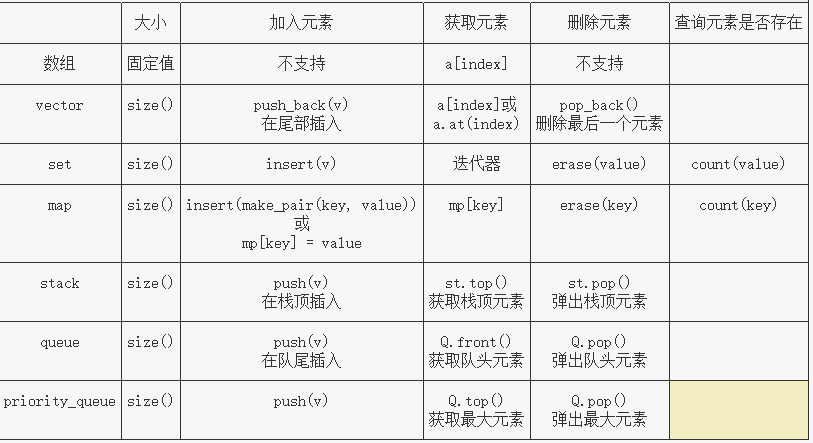
\includegraphics[height=6.5cm]{table.png}

\end{frame}

\begin{frame}
    \frametitle{作业}

    https://www.luogu.com.cn/contest/55131\\
    现在是答疑时间。


    

\end{frame}


\end{document}